\subsection{Implementation Plan}

intro: indipendenza dei moduli, unico constraint è prima Data4Help.

ordine dei sottosistemi: prima i back end e poi i front end in parallelo

ordine componenti:

\textbf{Data4Help}

\FloatBarrier
\begin{figure}[!h]
	\centering
	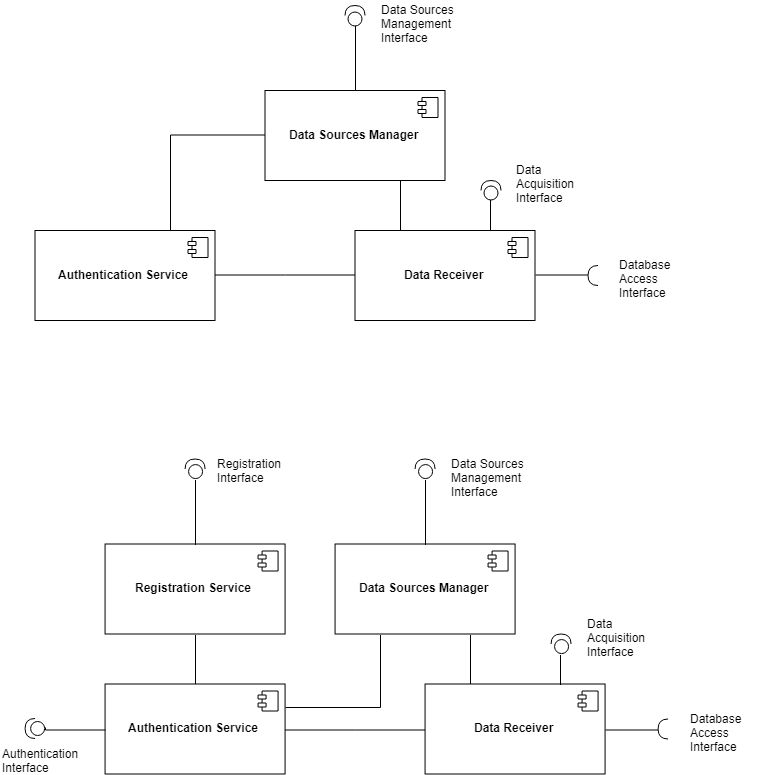
\includegraphics[width=\columnwidth]{d4h_dev_rcv.png}
	\caption{Data Acquisition Module development steps}
\end{figure}
 
\FloatBarrier

\FloatBarrier
\begin{figure}[!h]
	\centering
	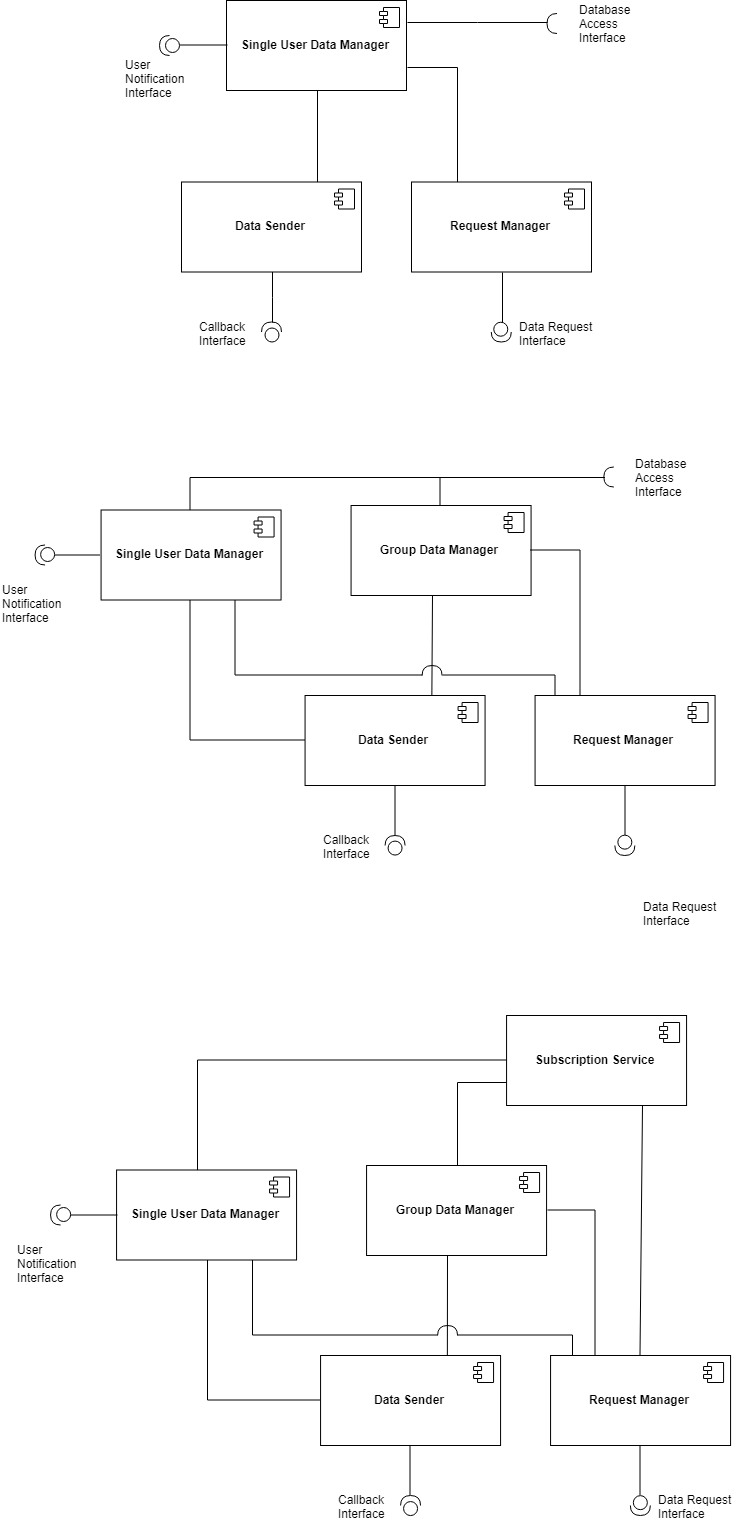
\includegraphics[ height=0.9\textheight]{d4h_dev_send.png}
	\caption{Data Request Module development steps}
\end{figure}

\FloatBarrier

\textbf{AutomatedSOS}
Prima BE, poi external Interfaces, poi FE

\textbf{Track4Run}
Prima BE, poi external Interfaces, poi FE

\subsection{Integration and Testing}
\subsubsection{Entry Criteria}
Percentuali (?)
Di base, quando i back end sono completati a meno di autenticazione

\subsubsection{Elements to be Integrated}

\FloatBarrier
\begin{figure}[!h]
	\centering
	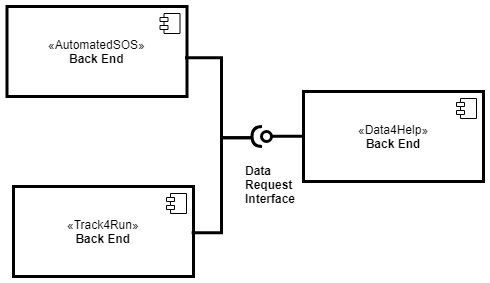
\includegraphics[width=0.7\columnwidth]{sysInt1.png}
	\caption{Step I - Back-ends integration}
\end{figure}

\FloatBarrier

\vspace{2px}
 
\FloatBarrier
\begin{figure}[!h]
	\centering
	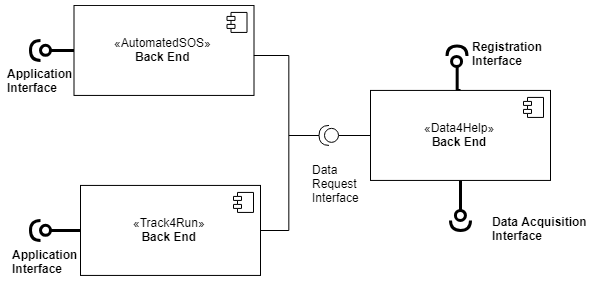
\includegraphics[width=\columnwidth]{sysInt2.png}
	\caption{Step II - External Interfaces integration}
\end{figure}

\FloatBarrier

\vspace{20px}

\FloatBarrier
\begin{figure}[!h]
	\centering
	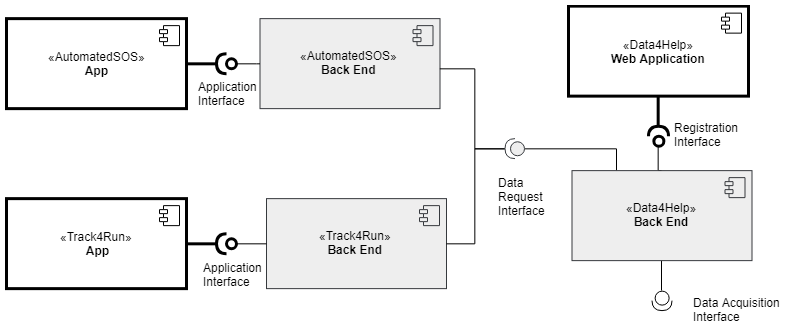
\includegraphics[width=\columnwidth]{sysInt3.png}
	\caption{Step III - Subsystems Front-ends integration}
\end{figure}

\FloatBarrier

\FloatBarrier
\begin{figure}[!h]
	\centering
	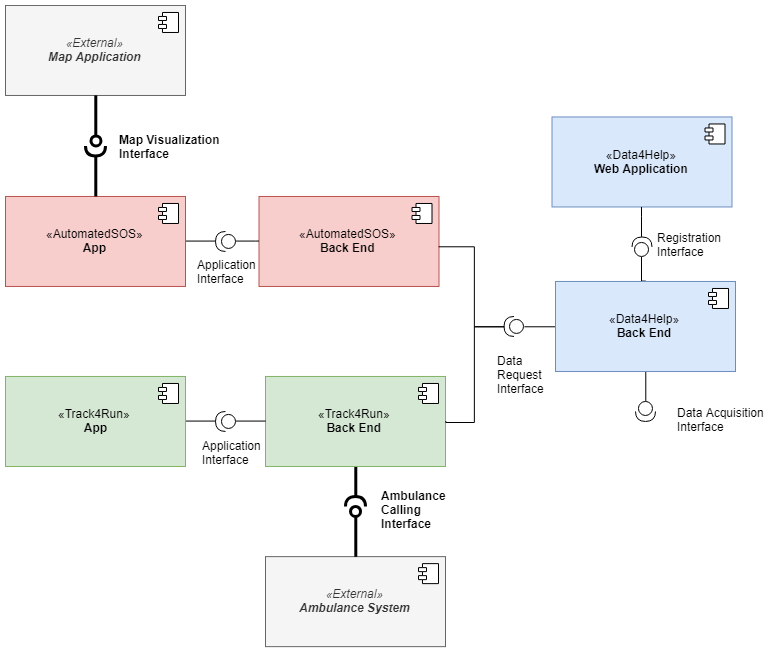
\includegraphics[width=\columnwidth]{sysInt4.png}
	\caption{Step IV - External Services integration}
\end{figure}

\FloatBarrier



\subsubsection{Integration Testing Strategy}
bottom up o continuous integration?

\subsubsection{Sequence of Component/Function Integration}

componente per componente
